\documentclass[a4paper,10pt,twocolumn]{article}
\usepackage[latin1]{inputenc}
\usepackage[english]{babel}
\usepackage{amsmath}
\usepackage{amsfonts}
\usepackage{amssymb}
\usepackage{titling}
\usepackage{nomencl}
\usepackage{booktabs}
\usepackage{graphicx}
\usepackage[style=ieee,backend=bibtex]{biblatex}
\usepackage{xspace}
\usepackage{fancyhdr}
\usepackage{varioref}
\usepackage[activate={true,nocompatibility},final,tracking=true,kerning=true,spacing=true,factor=1100,stretch=10,shrink=10]{microtype}
% activate={true,nocompatibility} - activate protrusion and expansion
% final - enable microtype; use "draft" to disable
% tracking=true, kerning=true, spacing=true - activate these techniques
% factor=1100 - add 10% to the protrusion amount (default is 1000)
% stretch=10, shrink=10 - reduce stretchability/shrinkability (default is 20/20)

% Path to images.
\graphicspath{{img/}}

% Setup nomenclature.
\makenomenclature
\newlength{\nomtitlesep}
\setlength{\nomtitlesep}{\nomitemsep}
\setlength{\nomitemsep}{-\parsep}
\renewcommand{\nomgroup}[1]{%
    \itemsep\nomtitlesep
    \ifthenelse{\equal{#1}{V}}{\item[\textbf{Variables}]}{}
    \itemsep\nomitemsep
}

% Setup bibiliography.
\addbibresource{bibliography}

% Document info.
\author{Z0966990}
\title{Regression Assignment}
\date{\today}

% Header and footer.
\pagestyle{fancy}
\fancyhf{}
\lhead{\thetitle}
\rhead{\theauthor}
\cfoot{\thepage}
\renewcommand{\headrulewidth}{0pt}
\renewcommand{\footrulewidth}{0pt}

% Macros
\newcommand{\MPG}{\textsc{mpg}\xspace}
\newcommand{\GPM}{\textsc{gpm}\xspace}
\newcommand{\VOL}{\textsc{vol}\xspace}
\newcommand{\HP}{\textsc{hp}\xspace}
\newcommand{\SP}{\textsc{sp}\xspace}
\newcommand{\WT}{\textsc{wt}\xspace}

\begin{document}
    
% Title page.
\begin{titlepage}
    \centering
    \vspace*{\fill}
    
\includegraphics[width=0.5\textwidth]{Durham}\\
    \vspace*{\fill}
    \LARGE\thetitle\\
    \large\theauthor\\
    \large L2 Engineering Mathematics\\
    \large\thedate\\
    \vspace*{\fill}
\end{titlepage}

% Nomenclature.
\nomenclature[0]{$R^2$}{Coefficient of determinability.}
\nomenclature[1]{$R^2_{adj}$}{Adjusted coefficient of determinability.}
\nomenclature[2]{$p$}{Number of parameters.}
\nomenclature[3]{$x$}{Predictor variables.}
\nomenclature[4]{$y$}{Explained variable.}
\nomenclature[5]{$\hat{y}$}{Estimate of explained variable.}
\nomenclature[6]{$\beta$}{Regression coefficents.}
\nomenclature[7]{$\hat{\beta}$}{Estimates of regression coefficents.}
\nomenclature[8]{$\epsilon$}{Random error.}

\nomenclature[V]{\MPG}{Fuel consumption in miles per gallon.}
\nomenclature[V]{\GPM}{Fuel consumption in gallons per mile.}
\nomenclature[V]{\HP}{Power output in horsepower.}
\nomenclature[V]{\SP}{Top speed in miles per hour.}
\nomenclature[V]{\WT}{Weight in pounds.}
\nomenclature[V]{\VOL}{Cab volume in cubic feet.}
\printnomenclature

% Main matter.
\section{Introduction}

Least squares regression was used to find the best linear model for predicting 
fuel consumption based on the properties of existing car models.

The dataset used to find the model came from a 1991 annual report on fuel 
economy for the US Environmental Protection Agency \cite{heavenrichlight}. The 
dataset specified the fuel consumption (\MPG) of 82 models of light vehicles 
alongside their power output (\HP), top speed (\SP), cab volume (\VOL) and 
weight (\WT). The models evaluated explained fuel consumption or its reciprocal 
(\GPM) as a function of the other four predictors specified in the dataset.

The scatter plots in Figure~\vref{fig:Data} indicated an inverse relationship 
between the explained variable \MPG and predictors \HP and \WT. For the same 
predictors, the variable \GPM suggested a linear relationship so was a 
better choice for the linear regression model used.

\begin{figure}[h]
    \centering
    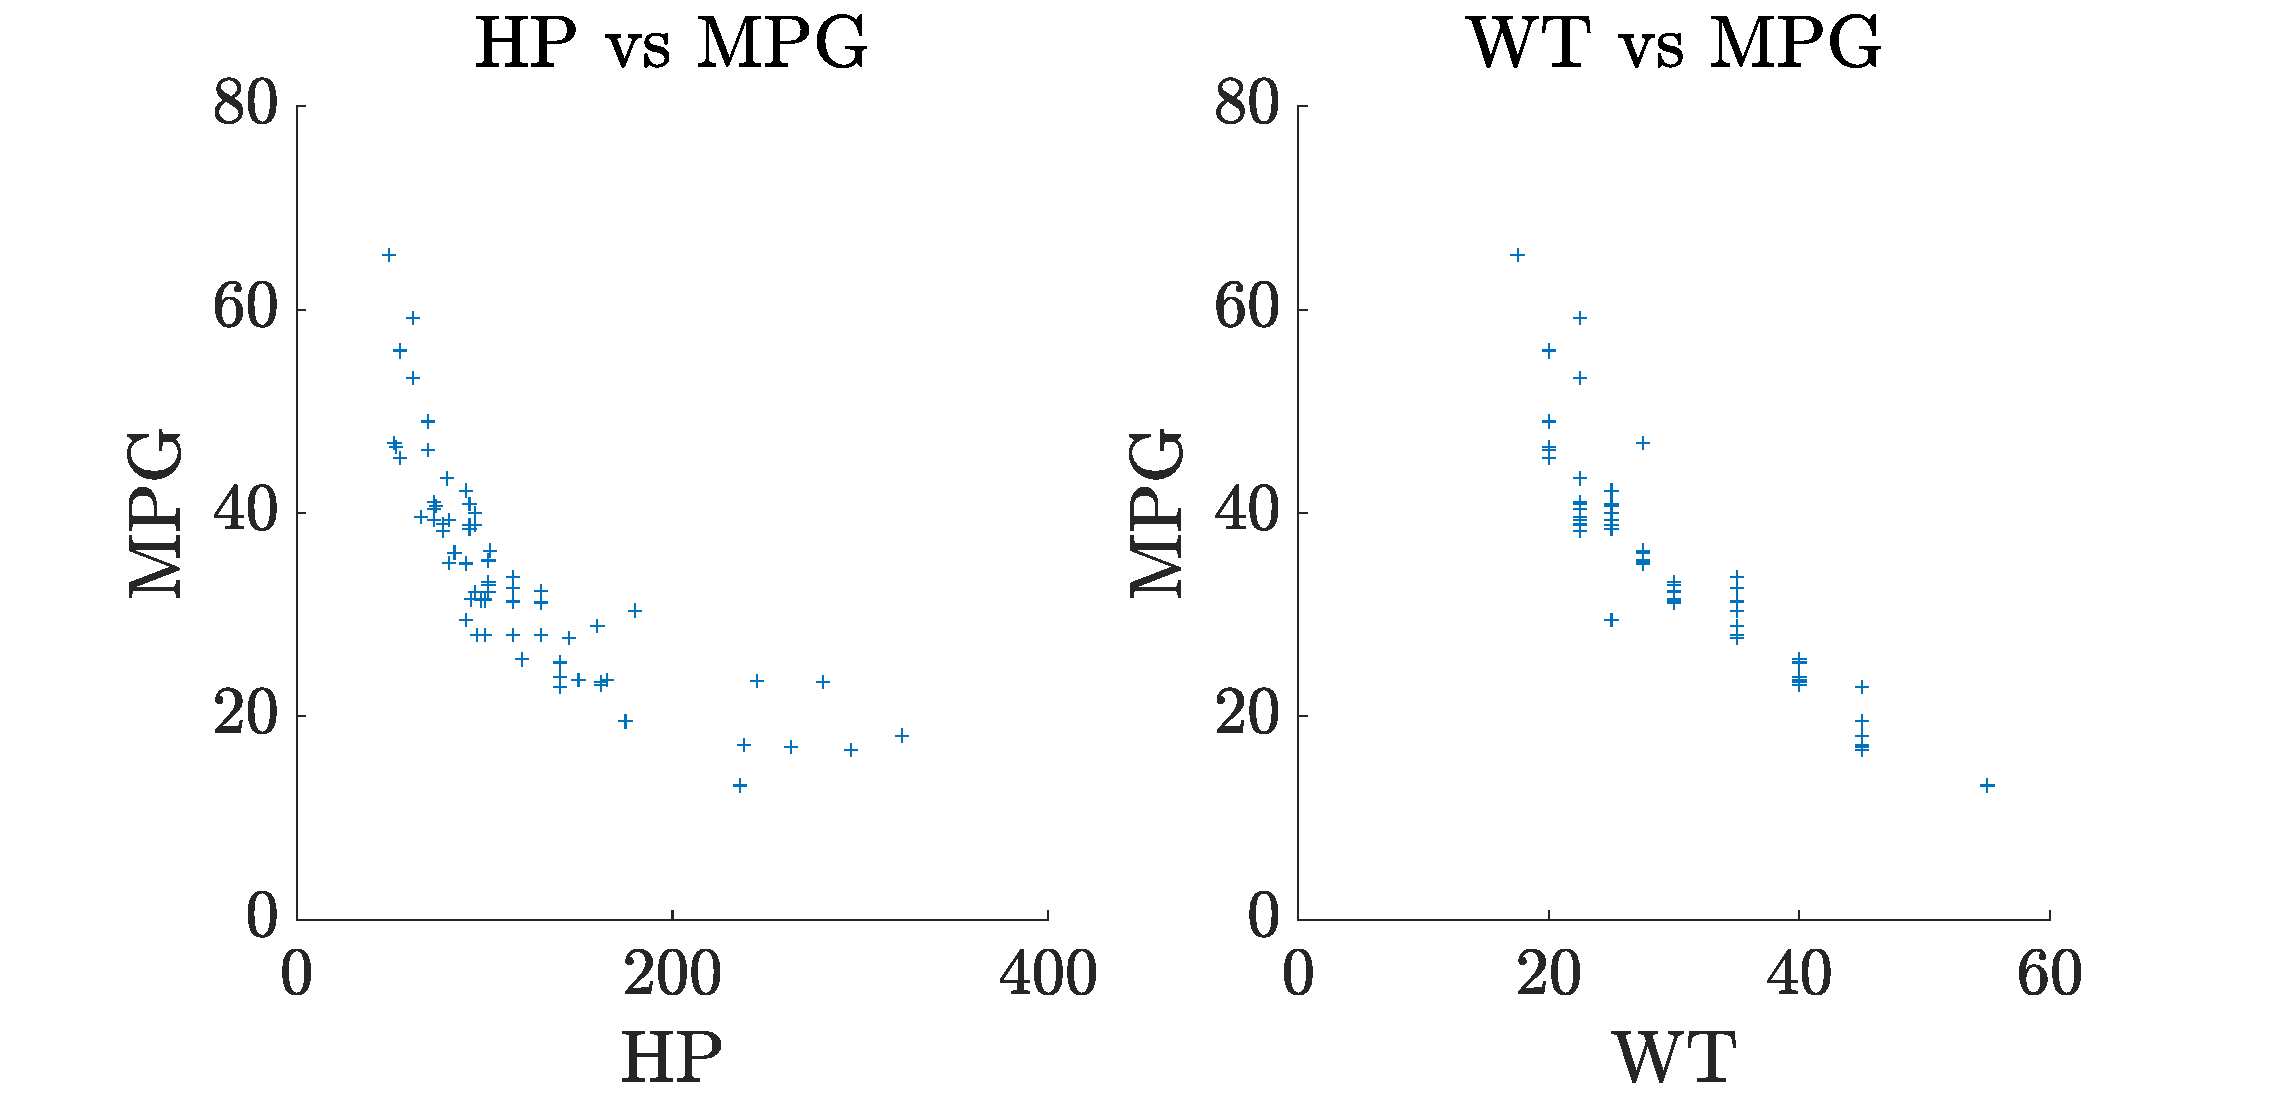
\includegraphics[width=0.42\textwidth]{MPG}
    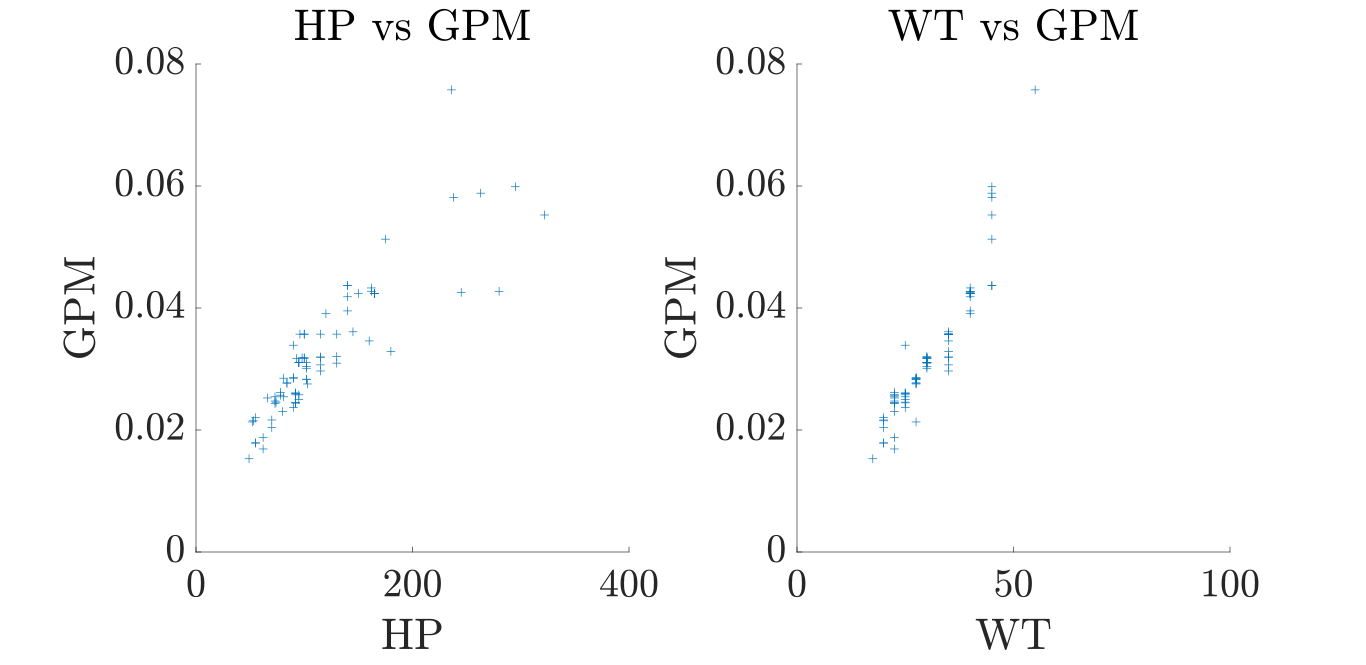
\includegraphics[width=0.42\textwidth]{GPM}
    \caption{Scatter plots of variables in the dataset.}
    \label{fig:Data}
\end{figure}

\section{Regression Modelling}

Before regression modelling could be performed, the following underlying 
conceptual multivariate linear model was chosen:

\begin{equation}
    y = \beta_0 + \beta_1 x_1 + ... + \beta_{p-1}x_{p-1} + \epsilon
    \label{eq:Model}
\end{equation}

The fuel economy dataset was used to find an estimate of this model, of the 
following form:

\begin{equation}
    \hat{y} = \hat{\beta}_0 + \hat{\beta}_1 x_1 + ... + \hat{\beta}_{p-1}x_{p-1}
    \label{eq:Estimate}
\end{equation}

Where $\hat{\beta}$ values are estimates of the regression coefficients chosen 
such that the prediction errors for the 82 makes of car in the dataset have the 
minimum variance. These residual errors are due to errors in the estimation of 
the regression coefficients and variation in the underlying data, $\epsilon$.

Different combinations of predictors \VOL, \HP, \SP and \WT were used to find 
models for predicting explained variables \MPG and \GPM.

These models were evaluated using the $R^2$ metric which describes what  
proportion of the variability in the residuals were due to the errors in 
estimating the regression coefficients, rather than variability in 
observations---$\epsilon$.

$R^2_{adj}$ additionally accounts for the additional degrees of freedom 
introduced by using multiple predictors. As the number of parameters increase, 
models become better at estimating the observed data by chance. This metric
reflects whether improvements are statistically significant and will generalise 
to new data.

The performance of each combination of predictors and explained variables 
modelled are listed in Table~\vref{table:Regression}. The $R^2_{adj}$ values 
show that the best model explained \GPM as a function of \VOL, \HP, \SP and 
\WT and the worst model explained \MPG as a function of \SP.

\begin{table*}
    \centering
    \begin{tabular}{lllllll}
    \toprule
    $y$ & $x_1, x_2, ..., x_{p-1}$ & $p$ & $R^2$ & $R^2_{adj}$ & K-S Test & K-S 
    $p$-value \\
    \midrule
    \MPG & \VOL, \HP, \SP, \WT & 5 & 0.87328 & 0.86670 & Pass & 0.51469 \\
    \MPG & \HP, \WT            & 3 & 0.82354 & 0.81908 & Fail & 0.011707 \\
    \MPG & \SP, \WT            & 3 & 0.82941 & 0.82510 & Fail & 0.018439 \\
    \MPG & \HP                 & 2 & 0.62387 & 0.61917 & Pass & 0.10995 \\
    \MPG & \SP                 & 2 & 0.47396 & 0.46738 & Pass & 0.41495 \\
    \MPG & \WT                 & 2 & 0.81918 & 0.81692 & Fail & 0.00088302 \\
    \GPM & \VOL, \HP, \SP, \WT & 5 & 0.91787 & 0.91361 & Pass & 0.075021 \\
    \GPM & \HP, \WT            & 3 & 0.91180 & 0.90957 & Pass & 0.11743 \\
    \GPM & \SP, \WT            & 3 & 0.90678 & 0.90442 & Fail & 0.038707 \\
    \GPM & \HP                 & 2 & 0.77135 & 0.76849 & Pass & 0.26418 \\
    \GPM & \SP                 & 2 & 0.56930 & 0.56391 & Pass & 0.46792 \\
    \GPM & \WT                 & 2 & 0.88116 & 0.87967 & Fail & 0.039028 \\
    \bottomrule
    \end{tabular}
    \caption{Comparison of performance of models with different variables.}
    \label{table:Regression}
\end{table*}
    
\section{Residual Analysis}

One way to envisage regression is to imagine a $p$ dimensional space with 
an axis for each variable. The linear model is a hyperplane which maps values 
for the prediction variables onto a value for the explained variable. The 
observed data for good regression models is normally distributed about that 
hyperplane with a small constant variance with respect to the predictor 
variables.

The Kolmogorov-Smirnov (K-S) test can be used to evaluate the normality of a 
dataset by standardising the dataset then performing a one sample test against 
the standard normal distribution. At the 5\% significance level, when the 
$p$-value is greater than 0.05 it becomes sufficiently unlikely that the 
dataset differs from the normal distribution.

In analysis, the K-S test was performed on the standardised residuals for the 
models in Table~\ref{table:Regression} and those models with sufficiently 
normal residuals at the 5\% significance level were marked with a pass 
alongside the $p$-value obtained. Normally distributed residuals suggest the 
observed data is normally distributed either side of the regression model.

\begin{figure}[h]
    \centering
    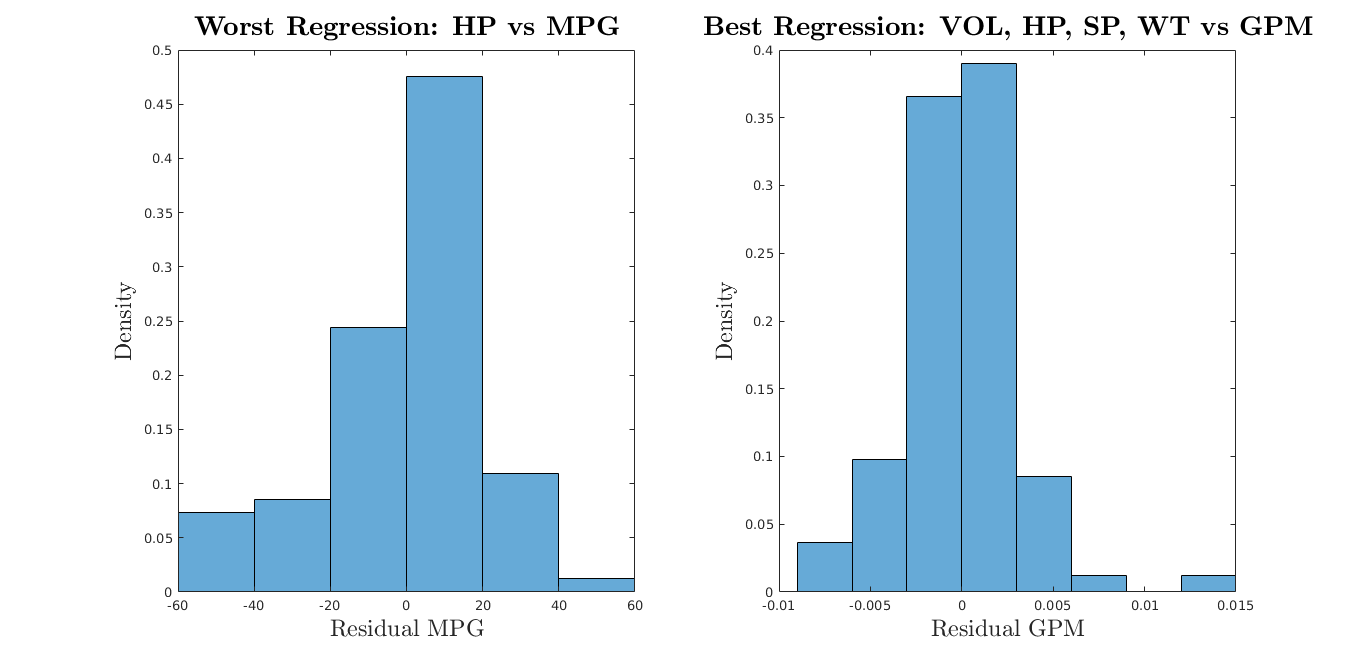
\includegraphics[width=0.42\textwidth]{Residuals}
    \caption{Residuals for regressions with worst and best $R^2_{adj}$.}
    \label{fig:Residuals}
\end{figure}

% References.
\printbibliography

\clearpage

\end{document}